% PATH GRAPHS

\documentclass[border=5, varwidth]{standalone}

\usepackage{tikz}

\begin{document}

    % ROUND 1
    Round 1:
    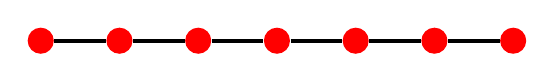
\begin{tikzpicture}[
            scale = 1,
            every node/.style={transform shape, text depth=0pt, circle},
            line/.style={line width = .05cm},
            ]
        
        \foreach \x in {0, ..., 6}
            \node[fill=red] (\x) at (\x, 0) {};
        
        \draw[line] (0) -- (1) -- (2) -- (3) -- (4) -- (5) -- (6);
    \end{tikzpicture}
    
    % ROUND 2
    Round 2:
    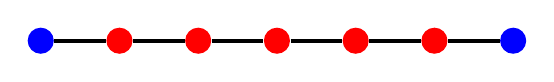
\begin{tikzpicture}[
            scale = 1,
            every node/.style={transform shape, text depth=0pt, circle},
            line/.style={line width = .05cm},
            ]
        
        \node[fill=blue] (0) at (0, 0) {};
        \node[fill=red] (1) at (1, 0) {};
        \node[fill=red] (2) at (2, 0) {};
        \node[fill=red] (3) at (3, 0) {};
        \node[fill=red] (4) at (4, 0) {};
        \node[fill=red] (5) at (5, 0) {};
        \node[fill=blue] (6) at (6, 0) {};
        
        \draw[line] (0) -- (1) -- (2) -- (3) -- (4) -- (5) -- (6);
    \end{tikzpicture}
    
    % ROUND 3
    Round 3:
    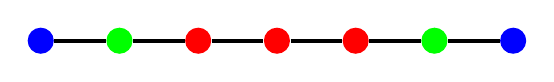
\begin{tikzpicture}[
            scale = 1,
            every node/.style={transform shape, text depth=0pt, circle},
            line/.style={line width = .05cm},
            ]
        
        \node[fill=blue] (0) at (0, 0) {};
        \node[fill=green] (1) at (1, 0) {};
        \node[fill=red] (2) at (2, 0) {};
        \node[fill=red] (3) at (3, 0) {};
        \node[fill=red] (4) at (4, 0) {};
        \node[fill=green] (5) at (5, 0) {};
        \node[fill=blue] (6) at (6, 0) {};
        
        \draw[line] (0) -- (1) -- (2) -- (3) -- (4) -- (5) -- (6);
    \end{tikzpicture}
    
    % ROUND 4
    Round 4:
    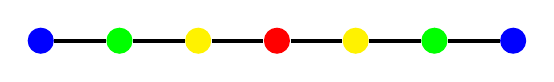
\begin{tikzpicture}[
            scale = 1,
            every node/.style={transform shape, text depth=0pt, circle},
            line/.style={line width = .05cm},
            ]
        
        \node[fill=blue] (0) at (0, 0) {};
        \node[fill=green] (1) at (1, 0) {};
        \node[fill=yellow] (2) at (2, 0) {};
        \node[fill=red] (3) at (3, 0) {};
        \node[fill=yellow] (4) at (4, 0) {};
        \node[fill=green] (5) at (5, 0) {};
        \node[fill=blue] (6) at (6, 0) {};
        
        \draw[line] (0) -- (1) -- (2) -- (3) -- (4) -- (5) -- (6);
    \end{tikzpicture}
    
    % ROUND 5
    Round 5:
    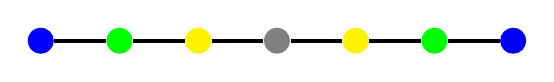
\begin{tikzpicture}[
            scale = 1,
            every node/.style={transform shape, text depth=0pt, circle},
            line/.style={line width = .05cm},
            ]
        
        \node[fill=blue] (0) at (0, 0) {};
        \node[fill=green] (1) at (1, 0) {};
        \node[fill=yellow] (2) at (2, 0) {};
        \node[fill=gray] (3) at (3, 0) {};
        \node[fill=yellow] (4) at (4, 0) {};
        \node[fill=green] (5) at (5, 0) {};
        \node[fill=blue] (6) at (6, 0) {};
        
        \draw[line] (0) -- (1) -- (2) -- (3) -- (4) -- (5) -- (6);
    \end{tikzpicture}
    
    
\end{document}